%  ╦┌┬┐┌─┐┬  ┌─┐┌┬┐┌─┐┌┐┌┌┬┐┌─┐┌─┐┬┌─┐┌┐┌
%  ║│││├─┘│  ├┤ │││├┤ │││ │ ├─┤│  ││ ││││
%  ╩┴ ┴┴  ┴─┘└─┘┴ ┴└─┘┘└┘ ┴ ┴ ┴└─┘┴└─┘┘└┘

\chapter{Implementación de los procedimientos de calibración}

En este capítulo se describe el desarrollo y arquitectura de software de las aplicaciones diseñadas para la calibración periódica de calibradores acústicos de acuerdo con la \mbox{IEC 60942}~\citeyearpar{IEC_TC29_2017} (tomando como base un modelamiento en GRAFCET) y de sonómetros de acuerdo con la norma \mbox{IEC 61672--3}~\citeyearpar{IEC_TC29_2013_1} (usando el sistema de reconocimiento de caracteres del capítulo~\ref{ch:image_recognition}).
El desarrollo del \emph{software} está publicado en el siguiente repositorio de GitHub:

    {\footnotesize\url{https://github.com/jfBranch/unal-acoustic-metrology.git}}


\section{Automatización de la calibración periódica de calibradores acústicos}
\label{sec:acoustic_calibrators_automation}
Siguiendo el método normalizado descrito en la sección~\ref{subsec:acoustic_calibrators_calibration_description} y el algoritmo de la figura~\ref{fig:acoustic_calibrator_calibration_flowchart}, se modeló la secuencia de calibración en un gráfico de etapas y transiciones explicado en la siguiente sección.

\subsection{GRAFCET descriptivo del proceso}
Para dar mayor claridad, en la figura~\ref{fig:GRAFCET_principal} se presenta la secuencia principal en la que se hacen llamadas a subrutinas mediante las etapas macro.
Los GRAFCET de las subrutinas se muestran en las figuras~\ref{fig:GRAFCET_micsens} a la~\ref{fig:GRAFCET_noise_dut}.
\vfill
\clearpage

\begin{figure}[!hp]
    \caption{GRAFCET de la rutina principal de la calibración periódica de calibradores acústicos.}
    \label{fig:GRAFCET_principal}
    \centering
    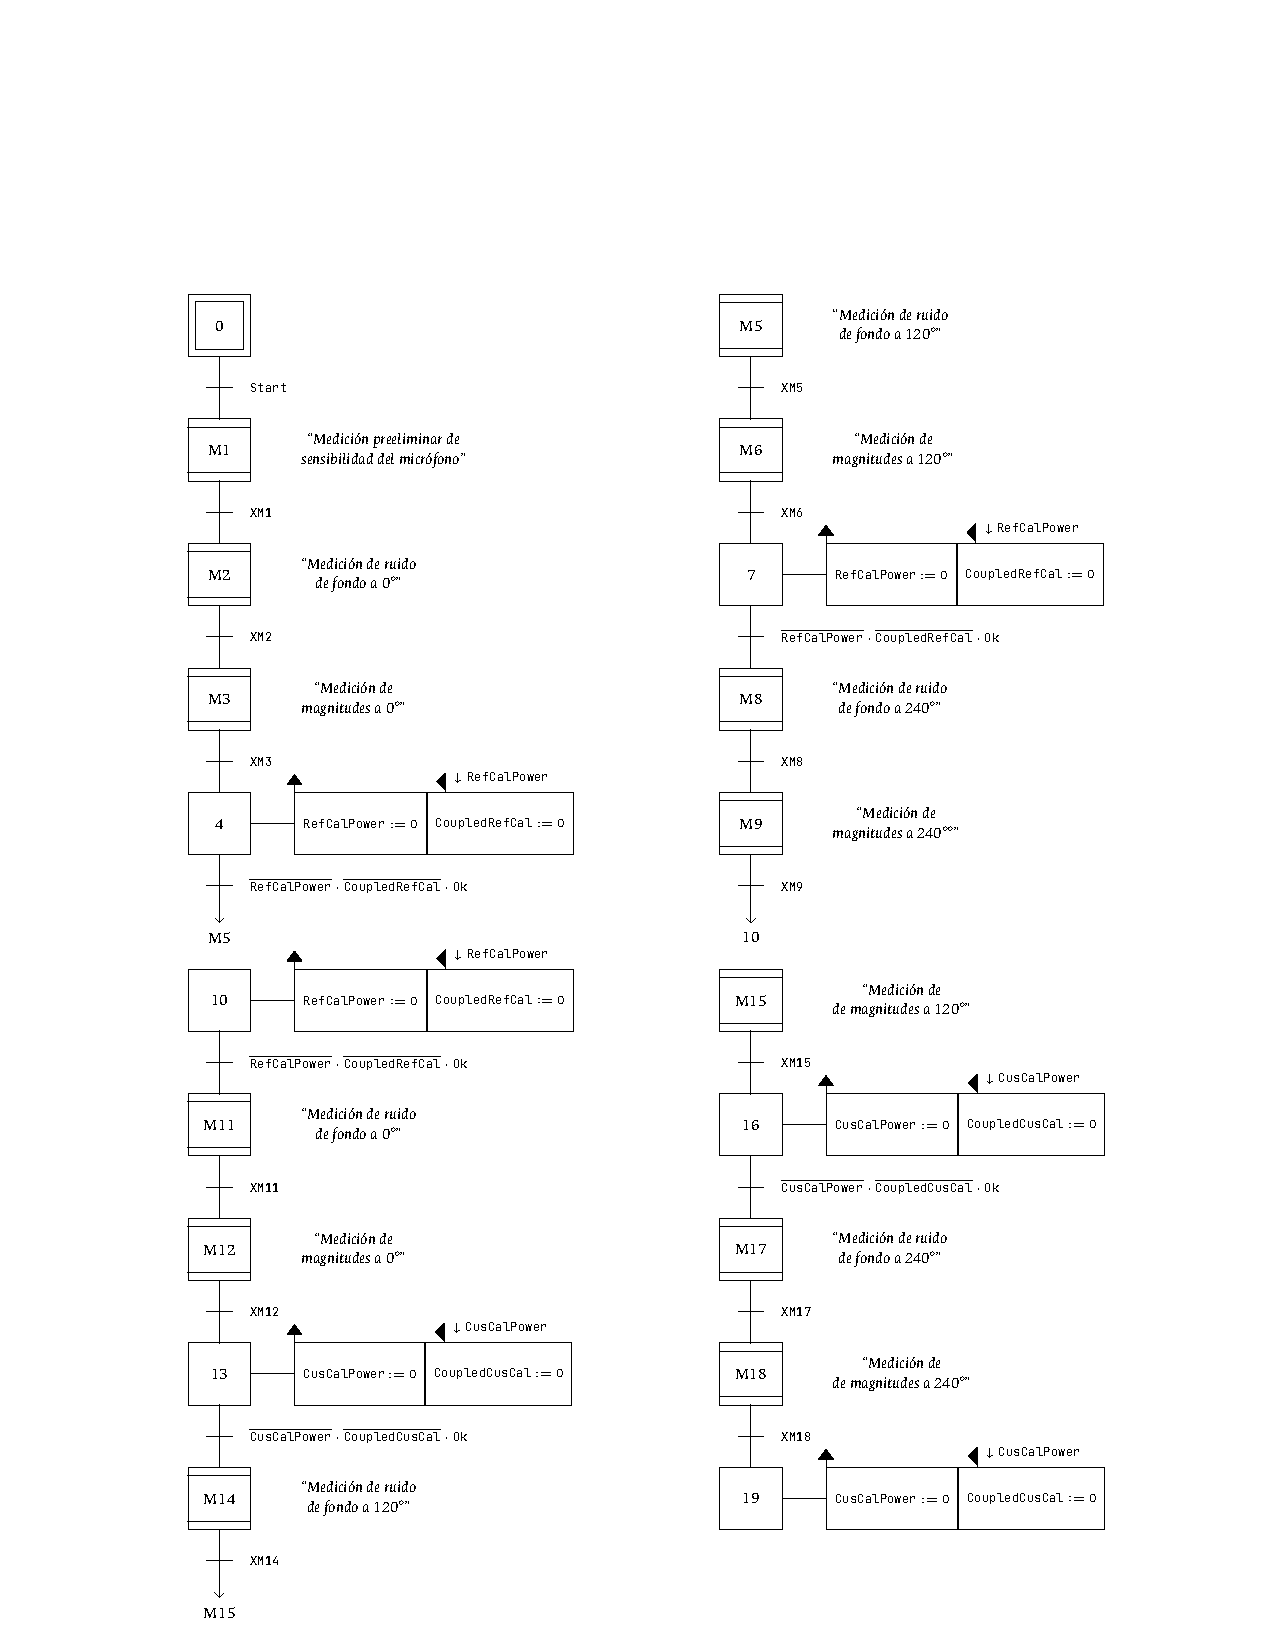
\includegraphics[height=0.92\textheight]{4_Implementación/principalGRAFCET}
    \caption*{\footnotesize Fuente: Elaboración propia.}
\end{figure}

En todos los GRAFCET, además de los operandos de cada etapa ({\scriptsize \texttt{X\#}}), se emplean los del siguiente cuadro:
%
\begin{table}[!h]
    \caption{Descripción de los operandos del GRAFCET de la secuencia principal.}
    \label{tab:principal_GRAFCET_operands}
    \centering
    \scriptsize
    \begin{tabularx}{\textwidth}{c|X}
        \hline
        \multicolumn{1}{c|}{\textbf{Operando}} & \multicolumn{1}{c}{\textbf{Descripción}}                                        \\ \hline
        {\tiny\texttt{RefCalOrient}}           & Orientación del calibrador acústico patrón.                                     \\ \hline
        {\tiny\texttt{RotatedRefCal}} & {\tiny\texttt{True}} si el calibrador patrón ya fue rotado o
            {\tiny\texttt{False}} si aún no ha sido rotado. \\ \hline
        {\tiny\texttt{RefCalPower}} & Estado del calibrador acústico patrón.
            {\tiny\texttt{True}} significa encender y
            {\tiny\texttt{False}}  es apagar.
        Esta acción es realizada manualmente por el operador. \\ \hline
        {\tiny\texttt{CoupledRefCal}} & Estado de acoplamiento del calibrador acústico patrón.
            {\tiny\texttt{True}} significa acoplar el calibrador al micrófono,
            {\tiny\texttt{False}}  es desacoplar el calibrador.
        Esta acción es realizada manualmente por el operador. \\ \hline
        {\tiny\texttt{CusCalOrient}}           & Orientación del calibrador acústico bajo prueba.                                \\ \hline
        {\tiny\texttt{RotatedCusCal}} & {\tiny\texttt{True}} si el calibrador bajo prueba ya fue rotado o
            {\tiny\texttt{False}} si aún no ha sido rotado. \\ \hline
        {\tiny\texttt{CusCalPower}} & Estado del calibrador acústico bajo calibración.
            {\tiny\texttt{True}} significa encender y
            {\tiny\texttt{False}}  es apagar.
        Esta acción es realizada manualmente por el operador. \\ \hline
        {\tiny\texttt{CoupledCusCal}} & Estado de acoplamiento del calibrador acústico bajo calibración.
            {\tiny\texttt{True}} significa acoplar el calibrador al micrófono,
            {\tiny\texttt{False}}  es desacoplar el calibrador.
        Esta acción es realizada manualmente por el operador. \\ \hline
        {\tiny\texttt{RepeatDialog}}           & Mostrar ventana emergente de diálogo con los botones ``Aceptar'' y ``Abortar''. \\ \hline
        {\tiny\texttt{Ok}} & Respuesta del usuario a un mensaje de diálogo con los botones ``Aceptar'' ({\tiny\texttt{True}})
        o ``Abortar'' ({\tiny\texttt{False}}). \\ \hline
        {\tiny\texttt{MeasMicSens}}            & Medir sensibilidad.
        Esta acción es automática.                                  \\ \hline
        {\tiny\texttt{MeasFinished}}           & Señal que indica que la medición en curso ha finalizado.                        \\ \hline
        {\tiny\texttt{MeasBackNoise}}          & Medir ruido de fondo.
        Esta acción es automática.                                \\ \hline
        {\tiny\texttt{MeasQuantities}}         & Medir magnitudes.
        Esta acción es automática.
    \end{tabularx}
\end{table}

\vfill
\clearpage

\subsection{Implementación en Python}
Si bien los GRAFCET's son empleados principalmente en aplicaciones mecánicas o eléctricas, es un lenguaje común que tiene el potencial para usarse como base para el desarrollo de software, dada su simplicidad y practicidad \citepalias{MHJSoftware2020}. A esto se suma la facilidad de aprenderlo, lo cual es una ventaja a la hora de integrar grupos de trabajo en los que participan personas de diferentes disciplinas.

\begin{figure}[!h]
    \centering
    \caption{Representación gráfica del paradigma \emph{Model-View-Controller}.}
    \label{fig:model_view_controller}
    \begin{tikzpicture}[thick, minimum width=2cm, minimum height=0.8cm]
        \node (model) at (0,0) [draw, process, fill=softOrange] {Modelo};
        \node (database) [below=1cm of model] {Base de datos};
        \node (databaseNortheast2) [above=0.15cm of database.north east,  inner sep=0pt, minimum size=0pt]{};
        \node (databaseNorthwest2) [above=0.15cm of database.north west,  inner sep=0pt, minimum size=0pt]{};
        \draw (database.north west) -- (database.south west)
        .. controls +(-30:0.2cm) and +(-150:0.2cm) .. (database.south east)
        -- (database.north east) .. controls +(-150:0.2cm) and +(-30: 0.2cm) .. (database.north west)
        -- (databaseNorthwest2.center) .. controls +(-30:0.2cm) and +(-150:0.2cm) .. (databaseNortheast2.center) -- (database.north east);
        \draw (databaseNorthwest2.center) .. controls +(30:0.2cm) and +(150:0.2cm) .. (databaseNortheast2.center);
        \node (database_north1) [above=0.2cm of database.north, inner sep=0pt, minimum size=0pt]{};
        \node (controller) [draw, process, fill=blue_sky, right=1cm of model]{Controlador};
        \node (view) [draw, process, fill=soft_red, right=1cm of controller]{Vista};
        \node (display) [draw, process, below=1cm of view]{};
        \node (displaySouthwest1) [below left=0.2cm and 0.2cm of display.south west, inner sep=0pt, minimum size=0pt]{};
        \node (displaySoutheast1) [below right=0.2cm and 0.2cm of display.south east, inner sep=0pt, minimum size=0pt]{};
        \draw (display.south west) -- (displaySouthwest1.center) -- (displaySoutheast1.center) -- (display.south east);
        \draw [-stealth] (database_north1) -- (model);
        \draw [stealth-stealth] (model) -- (controller);
        \draw [stealth-stealth] (controller) -- (view);
        \draw [stealth-stealth] (view) -- (display);
    \end{tikzpicture}
    \caption*{\footnotesize Fuente: Elaboración propia.}
\end{figure}
%
Normalmente, el diseño de un GRAFCET es llevado a la realidad en los sistemas empleando controladores lógicos programables (PLC), a los que están conectados los sensores y actuadores presentes en el sistema.
Sin embargo, en este desarrollo (siguiendo el paradigma de la programación orientada a objetos) la función del PLC es desempeñada \emph{virtualmente} por dos objetos cuyas clases están diseñadas para ser el controlador y el modelo en el patrón \emph{Model-View-Controller} (MVC), comúnmente utilizado en el desarrollo de aplicaciones web con interfaz gráfica (véase la figura~\ref{fig:model_view_controller}).
Para crear un entorno en el que estas interacciones virtuales puedan ocurrir, las clases de los objetos fueron diseñadas heredando de las clases {\small \texttt{QObject}} y {\small \texttt{QThread}} de la librería {\small \texttt{PyQt5}}, que permiten emplear la tecnología multi-hilos.
De manera que las señales y acciones ocurren en hilos paralelos según sea adecuado, sin \emph{congelar} el funcionamiento de la interfaz gráfica y permitiendo también el procesamiento en ``segundo plano''.
Las señales conectadas a los \emph{slots} son valores de progreso de la medición general o de la prueba en ejecución, y los valores de medición obtenidos en tiempo real.

La principal ventaja que se obtiene al usar un GRAFCET como base en el desarrollo de un \emph{software} que automatice las rutinas de un sistema, es que al final la programación queda encapsulada, ordenada e incluso etiquetada según las etapas del GRAFCET. De modo que esto facilita el diseño de la arquitectura de \emph{software} y permite que en la práctica se pueda ir a etapas específicas reutilizando las subrutinas, lo cual hace de esta una aplicación versátil e intuitiva para la calibración de calibradores acústicos.

\vfill

\begin{figure}[!hp]
    \caption{Diagrama de clases de la aplicación desarrollada para la calibración periódica de calibradores acústicos.}
    \label{fig:uml_acoustic_calibrators}
    \centering
    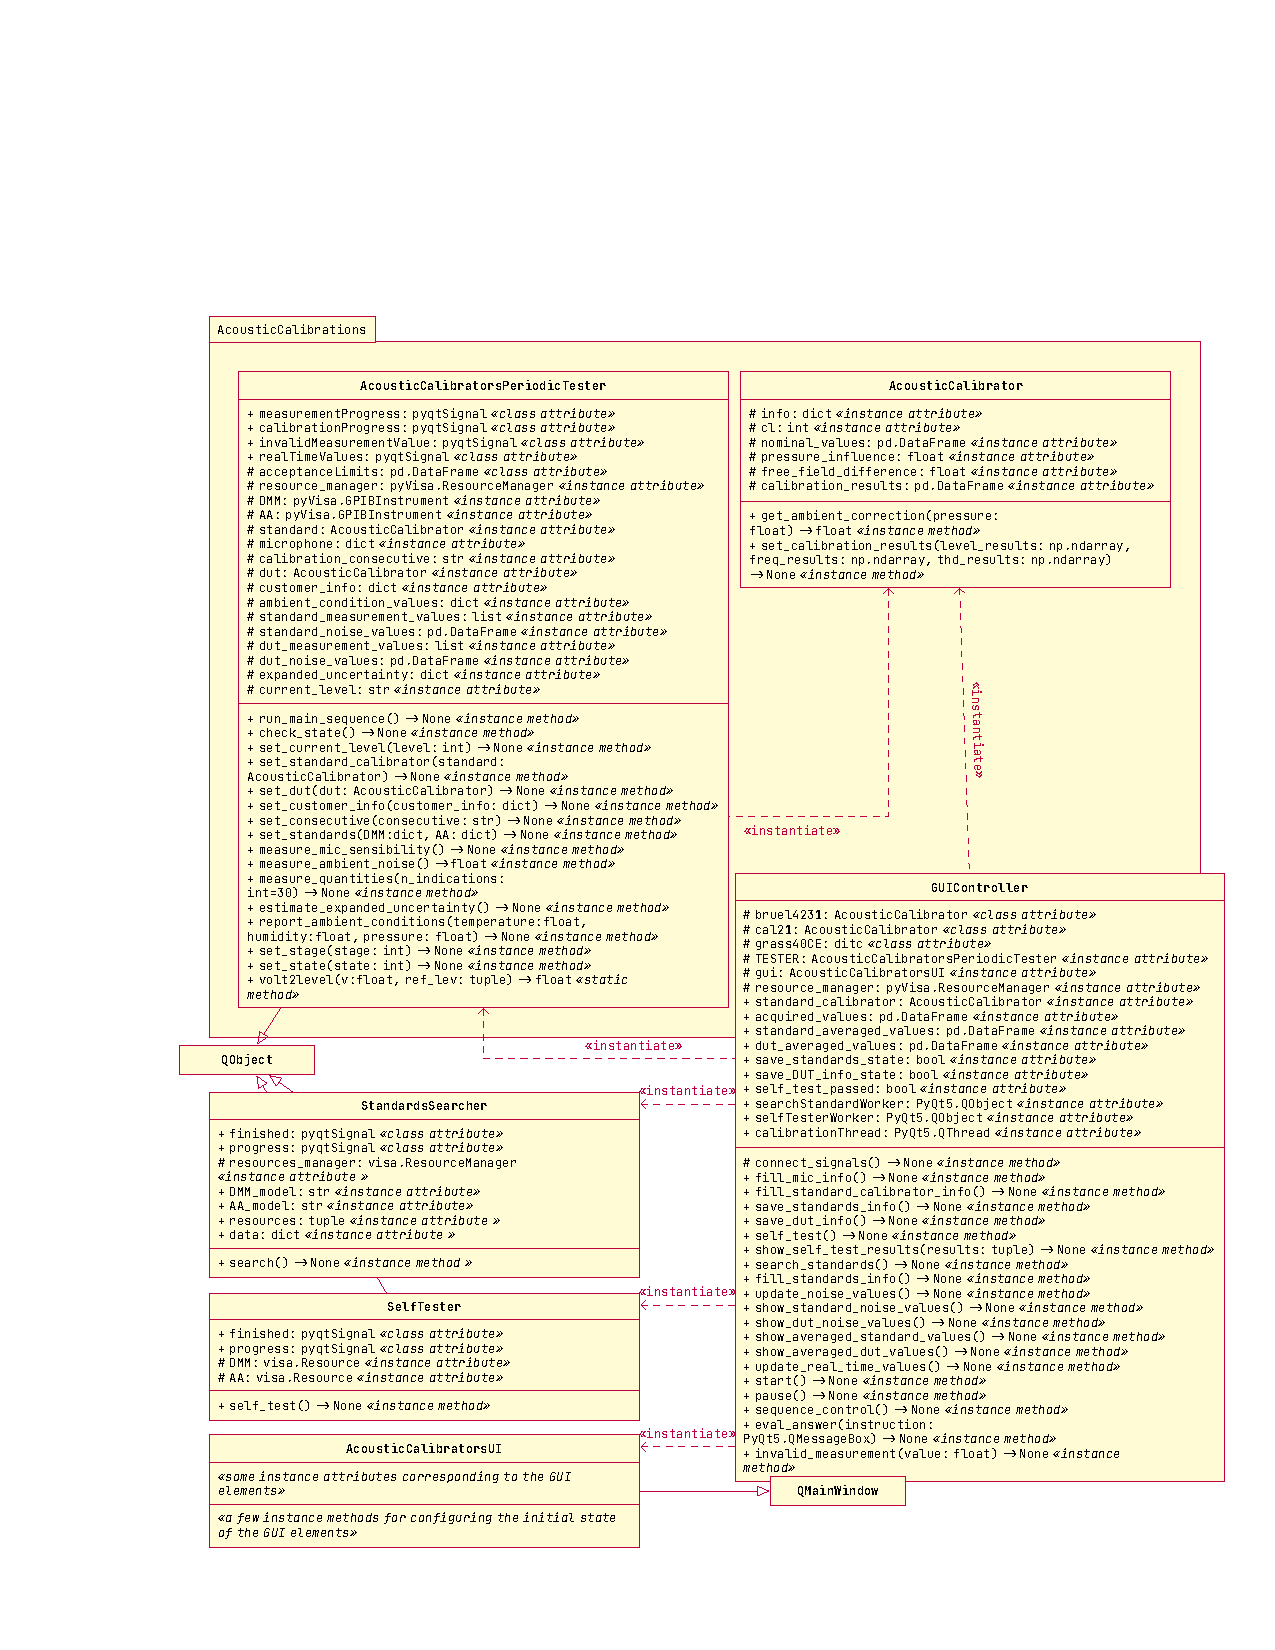
\includegraphics[width=\textwidth]{4_Implementación/IEC60942uml}
    \caption*{\footnotesize Fuente: Elaboración propia.}
\end{figure}

\subsubsection{Arquitectura de software}
%
El diagrama de clases de la figura~\ref{fig:uml_acoustic_calibrators} es un resumen de las clases principales (con sus atributos y métodos) diseñadas para el desarrollo de la aplicación para la calibración de calibradores acústicos.
También se presentan las clases heredadas y el instanciamiento entre clases.

La escritura del código se hizo aplicando las buenas prácticas de programación como: Documentación de clases, métodos e instrucciones relevantes, uso de atributos o métodos protegidos y las directrices de la guía PEP 8.
La interfaz gráfica se diseñó en Qt Designer de tal forma que se logre un manejo intuitivo de las funciones de la aplicación usando diferentes recursos como íconos, barras de progreso, menús desplegables, barra de herramientas, etc.
Con Qt Designer fue posible generar el código base de Python para el \emph{view} que lanza la aplicación y muestra la interfaz tal como fue diseñada.

\subsubsection{Descripción de funcionamiento}
\begin{figure}[!hb]
    \centering
    \caption{Interfaz gráfica de usuario de la aplicación para calibradores acústicos. Se muestra la pestaña de \emph{Patrones}.}
    \label{fig:calibrator_gui_standards}
    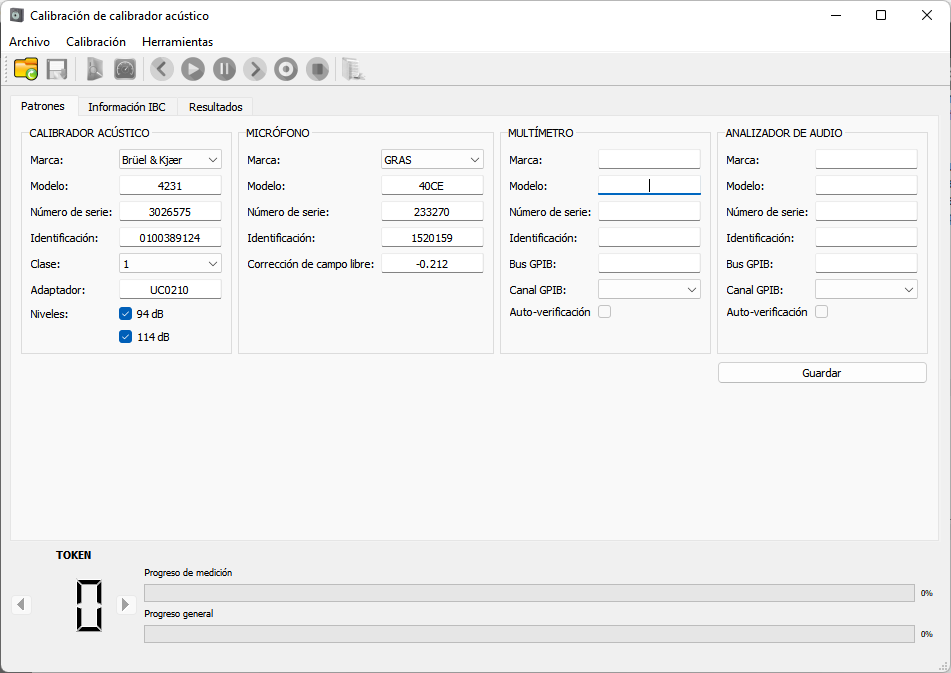
\includegraphics[width=0.8\textwidth]{4_Implementación/Figs/calibrator_gui_standards}
    \caption*{\footnotesize Fuente: Elaboración propia.}
\end{figure}
%
En la figura~\ref{fig:calibrator_gui_standards} se muestra la interfaz de usuario diseñada.
La pestaña de \emph{Patrones} es la mostrada en la vista inicial.
En esta, el usuario ingresa la información básica de los patrones empleados en la calibración.
Para el multímetro y el analizador de audio, si el usuario digita información en los campos de modelo, se habilita la herramienta 
\includegraphics[height=12pt]{4_Implementación/Figs/searchInstruments}, la cual busca automáticamente los modelos indicados entre todos los equipos disponibles conectados por GPIB al computador, extrae la información de estos y rellena los campos faltantes.

Una vez la información de los patrones está completa, el usuario puede hacer clic en \emph{Guardar}.
Se habilita la herramienta 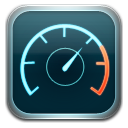
\includegraphics[height=12pt]{4_Implementación/Figs/test}, con la que se ejecuta la secuencia de auto-verificación de los patrones conectados por GPIB, si está disponible.
El resultado de la verificación se muestra en el \emph{check box} correspondiente.

\begin{figure}[!h]
    \centering
    \caption{Interfaz gráfica de usuario de la aplicación para calibradores acústicos. Se muestra la pestaña de \emph{Información IBC}.}
    \label{fig:calibrator_gui_dut}
    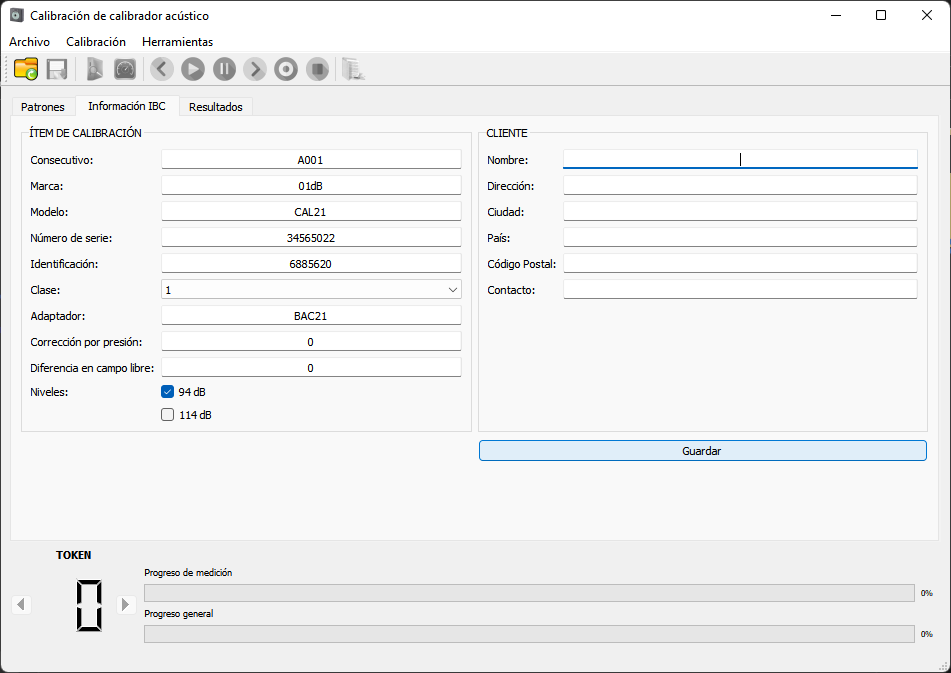
\includegraphics[width=0.8\textwidth]{4_Implementación/Figs/calibrator_gui_dut}
    \caption*{\footnotesize Fuente: Elaboración propia.}
\end{figure}

A continuación, en la pestaña \emph{Información IBC} (ver figura~\ref{fig:calibrator_gui_dut}), el usuario ingresa toda la información del calibrador bajo verificación y del cliente, necesaria para la calibración y para el certificado de calibración.
Cuando la información esté completa, el usuario puede hacer clic en \emph{Guardar} y, si el resultado de auto-verificación de los patrones fue correcto, entonces se habilita el botón 
\includegraphics[height=12pt]{4_Implementación/Figs/play}.
Al hacer clic en este se cumple la condición para la transición desde la etapa $0$ a la $1$ de la rutina principal del GRAFCET (figura~\ref{fig:GRAFCET_principal}).
En seguida se llevan a cabo todas las acciones de las demás etapas y, en la medida que avanza la secuencia, se van mostrando instrucciones al usuario para las acciones manuales y los resultados se presentan en tiempo real en la pestaña \emph{Resultados} de la siguiente figura.

\begin{figure}[!h]
    \centering
    \caption{Interfaz gráfica de usuario de la aplicación para calibradores acústicos. Se muestra la pestaña de \emph{Resultados}.}
    \label{fig:calibrator_gui_results}
    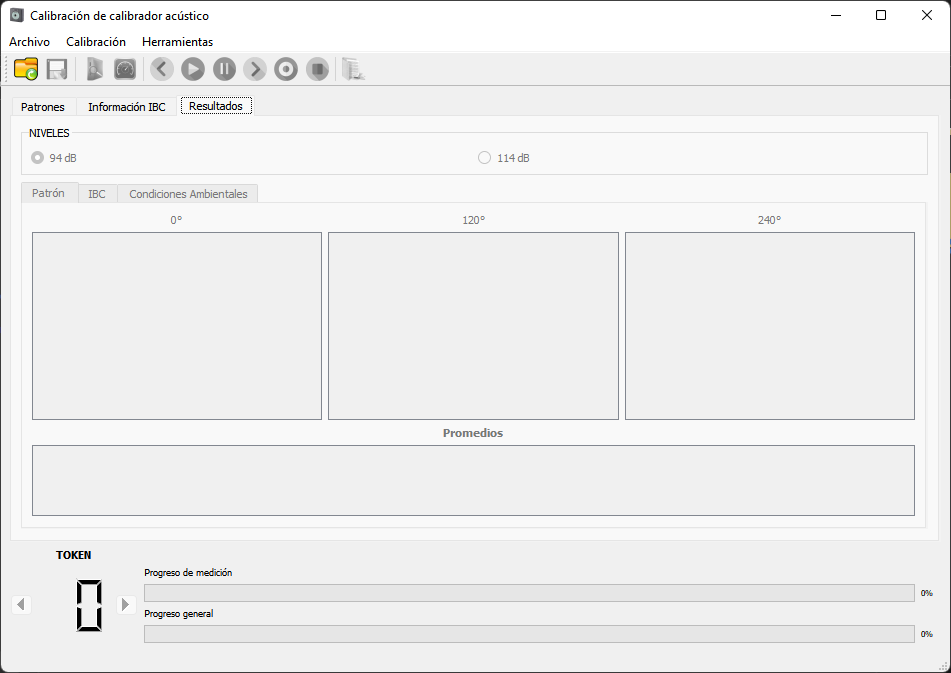
\includegraphics[width=0.8\textwidth]{4_implementación/Figs/calibrator_gui_results}
    \caption*{\footnotesize Fuente: Elaboración propia.}
\end{figure}

En la parte inferior de la ventana se incluye una barra de estado que indica la etapa actual (que tiene el \emph{token}), y dos barras de progreso, una para el progreso general de la calibración y otra para la medición en la etapa actual.
En cualquier momento de la calibración se puede hacer clic en 
\includegraphics[height=12pt]{4_Implementación/Figs/pause} para suspender temporalmente la secuencia y luego reanudarla haciendo clic nuevamente en 
\includegraphics[height=12pt]{4_Implementación/Figs/play}.
También se incluyen otros botones y herramientas en la interfaz, proyectando la aplicación a un desarrollo posterior que permita abrir y guardar sesiones de calibración, avanzar, retroceder etapas o ir a alguna específica del GRAFCET (inclusive generar automáticamente el certificado de calibración).


\section{Automatización de la calibración periódica de sonómetros}

De acuerdo con el método descrito en la sección~\ref{subsec:slm_calibration_description} y el diagrama de bloques de la figura~\ref{fig:slm_calibration_flowchart}, la aplicación se desarrolló con una metodología similar a la implementada para calibradores acústicos, como se explica en la siguiente sección.

\subsection{Implementación en Python}
El funcionamiento de la aplicación para calibradores acústicos asentó las bases para diseñar la aplicación para sonómetros.
Para aprovechar esas interacciones de los paradigmas \emph{model-view-controller} y GRAFCET que ocurren en el ambiente multihilos, se establecieron los siguientes pasos para la automatización de las pruebas realizadas en sonómetros;
estos pasos serían análogos a las etapas de un GRAFCET\@.

\begin{algorithm}[H]
    \caption{Pasos para la calibración periódica de sonómetros implementados en la aplicación desarrollada.}
    \label{alg:slm_calibration_steps}
    \scriptsize
    \DontPrintSemicolon
    \textbf{Paso 0.} Inicio, entrenar clasificador bayesiano. \;
    \textbf{Paso 1.} Verificar fuente de alimentación.\;
    \textbf{Paso 2.} Realizar prueba de indicación a la frecuencia de comprobación de la calibración.\;
    \textbf{Paso 3.} Verificar fuente de alimentación.\;
    \textbf{Paso 4.} Determinar el voltaje que produce una indicación del nivel de referencia.\;
    \textbf{Paso 5.} Realizar prueba de ponderación frecuencial $A$ con señales eléctricas.\;
    \textbf{Paso 6.} Realizar prueba de ponderación frecuencial $C$ con señales eléctricas.\;
    \textbf{Paso 7.} Realizar prueba de ponderación frecuencial $Z$ con señales eléctricas.\;
    \textbf{Paso 8.} Realizar prueba de ponderaciones frecuenciales a $\qty{1}{\kHz}$.\;
    \textbf{Paso 9.} Realizar prueba de ponderaciones temporales a $\qty{1}{\kHz}$.\;
    \textbf{Paso 10.} Realizar prueba de linealidad en el rango de niveles de referencia.\;
    \textbf{Paso 11.} Verificar fuente de alimentación.\;
    \textbf{Paso 12.} Fin\;
\end{algorithm}

%\begin{description}
%\item[Paso 0.] Inicio
%\item[Paso 1.] Verificar fuente de alimentación.
%\item[Paso 2.] Realizar prueba de indicación a la frecuencia de comprobación de la calibración.
%\item[Paso 3.] Verificar fuente de alimentación.
%\item[Paso 4.] Determinar el voltaje que produce una indicación del nivel de referencia.
%\item[Paso 5.] Realizar prueba de ponderación frecuencial $A$ con señales eléctricas.
%\item[Paso 6.] Realizar prueba de ponderación frecuencial $C$ con señales eléctricas.
%\item[Paso 7.] Realizar prueba de ponderación frecuencial $Z$ con señales eléctricas.
%\item[Paso 8.] Realizar prueba de ponderaciones frecuenciales a $\qty{1}{\kHz}$.
%\item[Paso 9.] Realizar prueba de ponderaciones temporales a $\qty{1}{\kHz}$.
%\item[Paso 10.] Realizar prueba de linealidad en el rango de niveles de referencia.
%\item[Paso 11.] Verificar fuente de alimentación.
%\item[Paso 12.] Fin
%\end{description}

Además de los hilos en los que el modelo hace sus operaciones y la vista envía y recibe las instrucciones del controlador, para esta aplicación fueron necesarios dos hilos más: uno que captura y muestra las imágenes del objeto de vídeo y otro que en segundo plano procesa, reconoce y guarda en disco en formato binario las imágenes de cada punto de calibración.
Todo esto a la vez que el modelo está corriendo temporizadores, enviando instrucciones a los instrumentos patrones y haciendo cálculos.
También se agregan otras señales Qt para indicar el arranque y parada de temporizadores, entregar el cuadro de vídeo capturado, indicar la liberación del objeto de vídeo y la finalización de guardado del vídeo, y enviar los mensajes de \emph{logging}.

Asignar los procesos de cálculo de los voltajes de prueba y temporizadores que se realizan en el modelo, y los procesos de reconocimiento de imágenes a hilos separados es un beneficio para el mantenimiento del \emph{software} y el desempeño de la aplicación.
Por ejemplo, el último objetivo de este proyecto, que consiste en el modelamiento de las cadenas de Markov, se puede implementar como un proceso adicional en el hilo de reconocimiento de imágenes, sin afectar los otros procesos.

\vfill

\begin{figure}[!hp]
    \caption{Diagrama de clases de la aplicación desarrollada para la calibración periódica de sonómetros.}
    \label{fig:uml_sonometers}
    \centering
    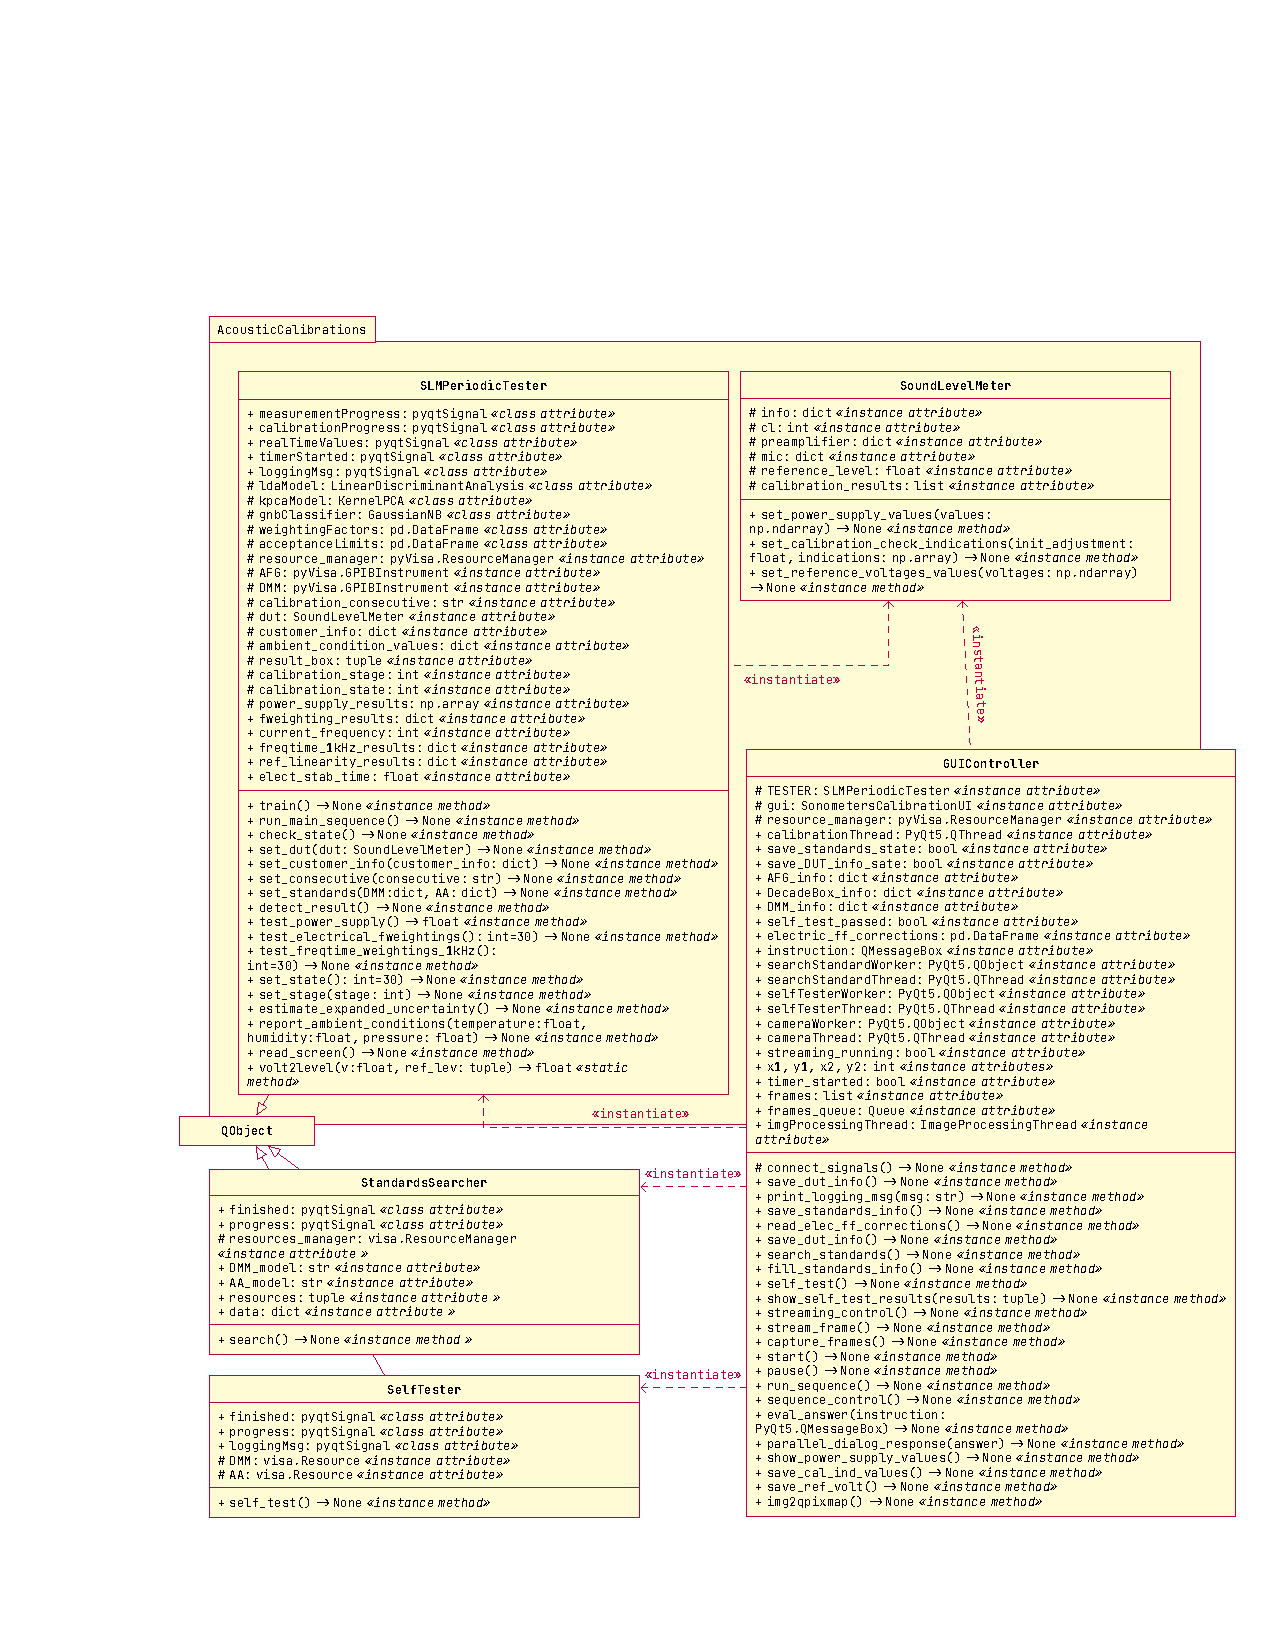
\includegraphics[width=\textwidth]{4_Implementación/IEC61672uml}
    \caption*{\footnotesize Fuente: Elaboración propia.}
\end{figure}
%
\begin{figure}[!h]
    \ContinuedFloat
    \centering
    \caption{Diagrama de clases de la aplicación desarrollada para la calibración periódica de sonómetros. (Continuación)}
    \begin{tikzpicture}[font=\tiny\ttfamily]
        \begin{class}[text width=1.6cm]{QMainWindow}{-1,0.9}\end{class}

        \begin{class}[text width=8cm]{SoundLevelMetersUI}{-1,0}
            \inherit{QMainWindow}
            \attribute{\textit{\guillemotleft some instance attributes corresponding to the GUI elements\guillemotright}}
            \operation{\textit{\guillemotleft a few instance methods for configuring the initial state of the GUI elements\guillemotright}}
        \end{class}

        \begin{class}[text width=4cm]{GUIController}{8,0}
            \attribute{\textit{\guillemotleft same attributes\guillemotright}}
            \operation{\textit{\guillemotleft same methods\guillemotright}}
        \end{class}

        \node (ACUINorth1)[below=0.2 of SoundLevelMetersUI.north east, inner sep=0pt, minimum size=0pt]{};
        \node (GUICWest4)[right=2.6 of ACUINorth1, inner sep=0pt, minimum size=0pt]{};
        \draw [umlcd style dashed line, <-] (ACUINorth1) -- node[pos=0.5,above,sloped]{\guillemotleft instantiate\guillemotright} (GUICWest4);

        \begin{class}[text width=2cm]{QObject}{-3,-4.5}\end{class}

        \begin{class}[text width=6cm]{VideoObject}{2, -2}
            \inherit{QObject}
            \attribute{+ frameCaptured: pyqtSignal \textit{\guillemotleft class attribute\guillemotright}}
            \attribute{+ cameraReleased: pyqtSignal \textit{\guillemotleft class attribute\guillemotright}}
            \attribute{+ loggingMsg: pyqtSignal \textit{\guillemotleft class attribute\guillemotright}}
            \attribute{+ run\_flag: bool \textit{\guillemotleft instance attribute\guillemotright}}
            \attribute{+ fps: int \textit{\guillemotleft instance attribute\guillemotright}}
            \attribute{+ frame\_size: tuple \textit{\guillemotleft instance attribute\guillemotright}}

            \operation{+ run() ->\,None \textit{\guillemotleft instance method\guillemotright}}
        \end{class}

        \begin{class}[text width=6cm]{VideoSaving}{2, -4.9}
            \inherit{QObject}
            \attribute{+ videoSaved: pyqtSignal \textit{\guillemotleft class attribute\guillemotright}}
            \attribute{+ loggingMsg: pyqtSignal \textit{\guillemotleft class attribute\guillemotright}}
            \attribute{+ frames: list \textit{\guillemotleft instance attribute\guillemotright}}
            \attribute{+ video\_writer: cv.VideoWriter \textit{\guillemotleft instance attribute\guillemotright}}

            \operation{+ save\_video() ->\,None \textit{\guillemotleft instance method\guillemotright}}
        \end{class}

        \begin{class}[text width=2cm]{QThread}{-3,-9}\end{class}

        \begin{class}[text width=6cm]{ImageProcessingThread}{2, -7.5}
            \inherit{QThread}
            \attribute{+ realTimeValues: pyqtSignal \textit{\guillemotleft class attribute\guillemotright}}
            \attribute{+ loggingMsg: pyqtSignal \textit{\guillemotleft class attribute\guillemotright}}
            \attribute{\# frames\_queue: Queue \textit{\guillemotleft instance attribute\guillemotright}}
            \attribute{\# TESTER: SLMPeriodicTester \textit{\guillemotleft instance attribute\guillemotright}}
            \attribute{\# stage: int \textit{\guillemotleft instance attribute\guillemotright}}
            \attribute{\# current\_f: int \textit{\guillemotleft instance attribute\guillemotright}}
            \attribute{\# fweightings: list \textit{\guillemotleft instance attribute\guillemotright}}
            \attribute{\# octave\_frequencies: list \textit{\guillemotleft instance attribute\guillemotright}}
            \attribute{+ fps: int \textit{\guillemotleft instance attribute\guillemotright}}

            \operation{+ run() ->\,None \textit{\guillemotleft instance method\guillemotright}}
        \end{class}

        \draw [umlcd style dashed line, <-](VideoObject.east) -| node[pos=0.3,above,sloped]{\guillemotleft instantiate\guillemotright} (GUIController.south);
        \draw [umlcd style dashed line, <-](VideoSaving.east) -| node[pos=0.3,above,sloped]{\guillemotleft instantiate\guillemotright} (GUIController.south);
        \draw [umlcd style dashed line, <-](ImageProcessingThread.east) -| node[pos=0.3,above,sloped]{\guillemotleft instantiate\guillemotright} (GUIController.south);
    \end{tikzpicture}
    \caption*{\footnotesize Fuente: Elaboración propia.}
\end{figure}

\subsubsection{Arquitectura de software}
El diagrama de clases de la figura~\ref{fig:uml_sonometers} es un resumen de las clases principales (con sus atributos y métodos) diseñadas para el desarrollo de la aplicación para la calibración de sonómetros.
También se presentan las clases heredadas y el instanciamiento entre clases.

La escritura del código se hizo aplicando las buenas prácticas de programación como: Documentación de clases, métodos e instrucciones relevantes, uso de atributos o métodos protegidos, aseguramiento de recursos para evitar condiciones de carrera entre hilos, colas para el procesamiento en segundo plano y las directrices de la guía PEP 8.
La interfaz gráfica se diseñó en Qt Designer de tal forma que se logre un manejo intuitivo de las funciones de la aplicación usando diferentes recursos como íconos, barras de progreso, menús desplegables, barra de herramientas, etc.
Con Qt Designer fue posible generar el código base de Python para el \emph{view} que lanza la aplicación y muestra la interfaz tal como fue diseñada.

\subsubsection{Descripción de funcionamiento}

\begin{figure}[!h]
    \centering
    \caption{Interfaz gráfica de usuario de la aplicación para sonómetros. Se muestra la pestaña de \emph{Patrones}.}
    \label{fig:slm_gui_standards}
    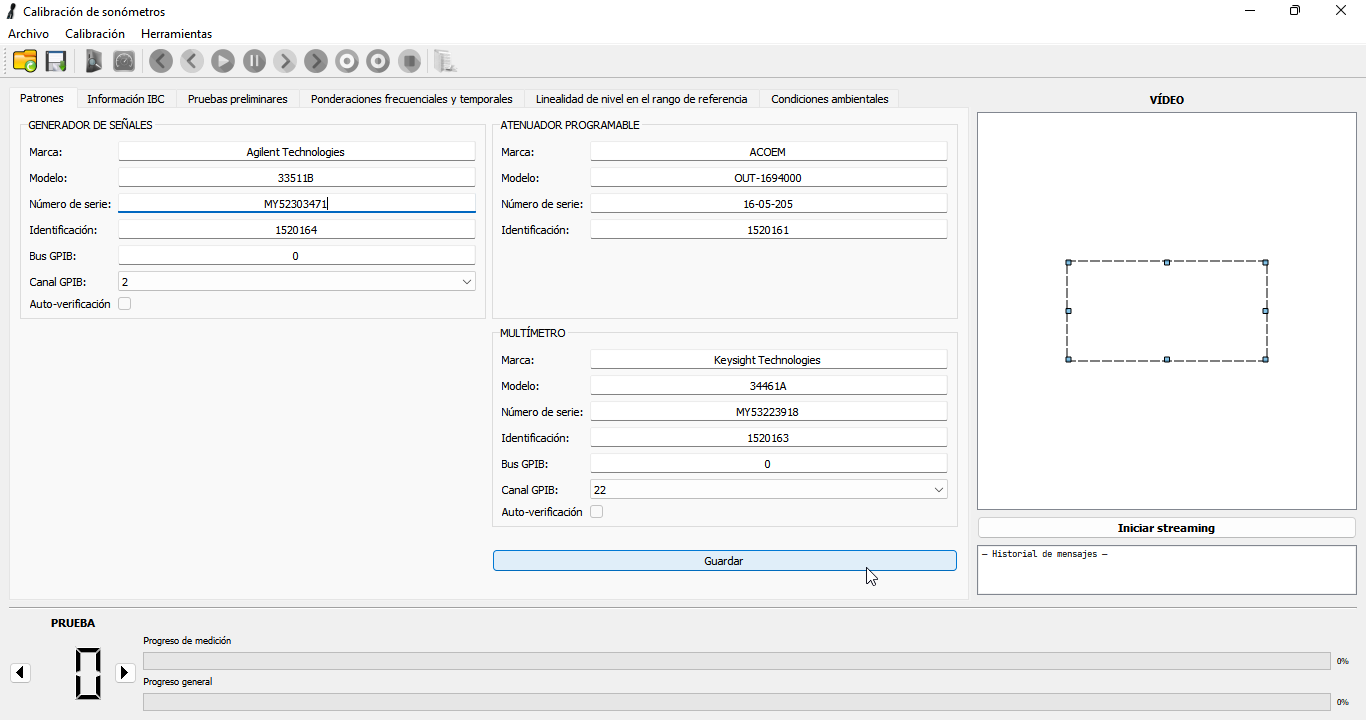
\includegraphics[width=\textwidth]{4_implementación/Figs/slm_gui_standards}
    \caption*{\footnotesize Fuente: Elaboración propia.}
\end{figure}

La aplicación para la calibración de sonómetros tiene un flujo de trabajo similar a la de calibradores acústicos.
En la figura~\ref{fig:slm_gui_standards} se muestra la interfaz gráfica de usuario diseñada.
En la vista inicial, la pestaña de \emph{Patrones} es la primera en mostrarse.
En esta, el usuario ingresa la información básica de los patrones empleados en la calibración.
Para el generador de señales y el multímetro digital, si el usuario digita información en los campos de modelo, se habilita la herramienta 
\includegraphics[height=12pt]{4_Implementación/Figs/searchInstruments}, la cual busca automáticamente los modelos indicados entre todos los equipos disponibles conectados por GPIB al computador, extrae la información de estos y rellena los campos faltantes.

Una vez la información de los patrones está completa, el usuario puede hacer clic en \emph{Guardar}.
Se habilita la herramienta 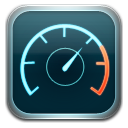
\includegraphics[height=12pt]{4_Implementación/Figs/test}, con la que se ejecuta la secuencia de auto-verificación de los patrones conectados por GPIB, si está disponible.
El resultado de la verificación se muestra en el \emph{check box} correspondiente.

Dado que en esta aplicación se realizan más tareas y hay mayor interacción de los hilos de programación, fue conveniente incluir un {\footnotesize \texttt{QListWidget}} en el que se indexan registros de eventos con su correspondiente marca de tiempo, usando un código de colores (negro: mensaje informativo, verde: acción importante realizada y rojo: error o acción finalizada incorrectamente).
Este registro de eventos está siempre visible debajo del recuadro al que se transmiten los cuadros de vídeo.

\begin{figure}[!h]
    \centering
    \caption{Interfaz gráfica de usuario de la aplicación para sonómetros. Se muestra la pestaña de \emph{Información del IBC}.}
    \label{fig:slm_gui_dut}
    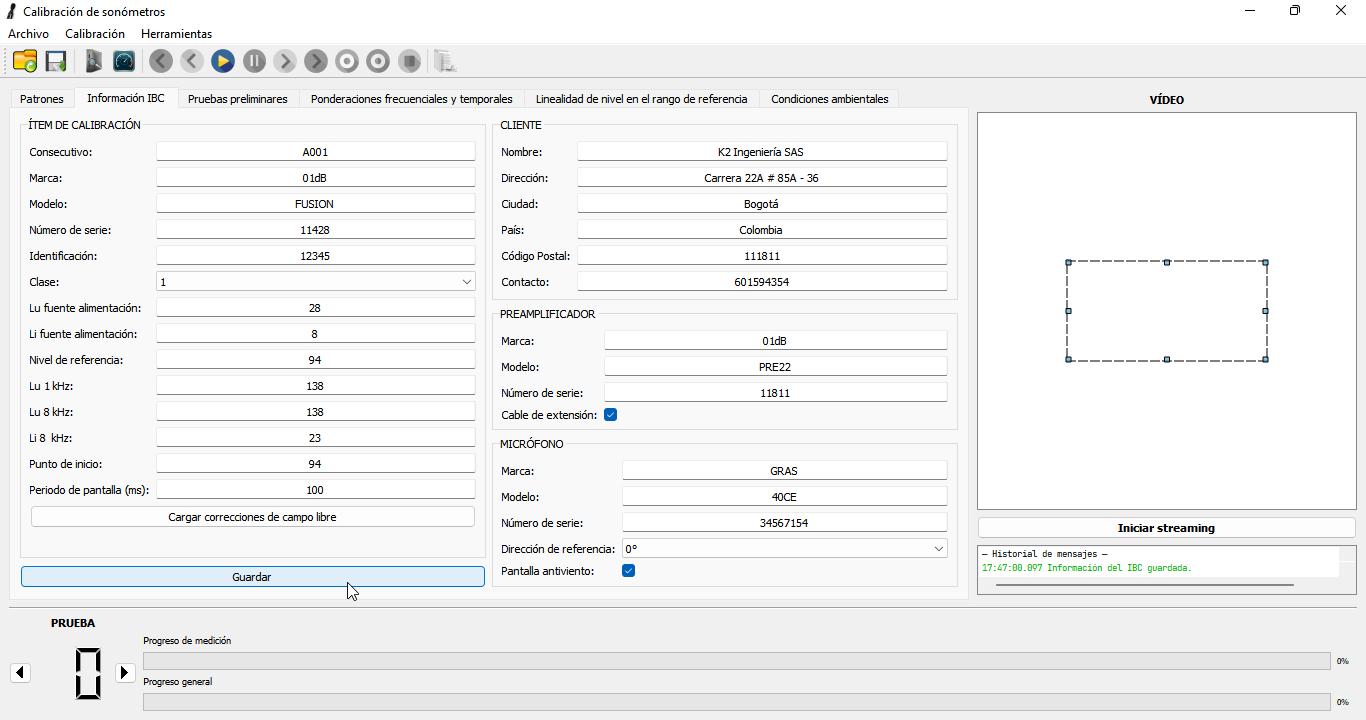
\includegraphics[width=\textwidth]{4_implementación/Figs/slm_gui_dut}
    \caption*{\footnotesize Fuente: Elaboración propia.}
\end{figure}

A continuación, en la pestaña \emph{Información IBC} (véase figura~\ref{fig:slm_gui_dut}), el usuario ingresa toda la información del sonómetro bajo verificación y del cliente, necesaria para la calibración y para el certificado de calibración.
Cuando la información esté completa, el usuario puede hacer clic en \emph{Guardar}.
Según la configuración indicada para el sonómetro, el programa buscará en una base de datos los factores de corrección de campo libre;
si estos no están disponibles, entonces el usuario puede crear un archivo separado por comas con los factores de corrección y cargarlos manualmente.
Luego, si el resultado de auto-verificación de los patrones fue correcto, entonces se habilita el botón 
\includegraphics[height=12pt]{4_Implementación/Figs/play}.
Al hacer clic en este se ejecuta el paso $0$ del algoritmo~\ref{alg:slm_calibration_steps}.
En seguida se llevan a cabo todas las acciones de los demás pasos y, en la medida que avanza la secuencia, se van mostrando instrucciones al usuario para las acciones manuales (ver figura~\ref{fig:slm_gui_results1}).

\vfill
\clearpage

\begin{figure}[!h]
    \centering
    \caption{Interfaz gráfica de usuario de la aplicación para sonómetros. Se muestra la pestaña de \emph{Pruebas preliminares} y un cuadro de diálogo con una instrucción.}
    \label{fig:slm_gui_results1}
    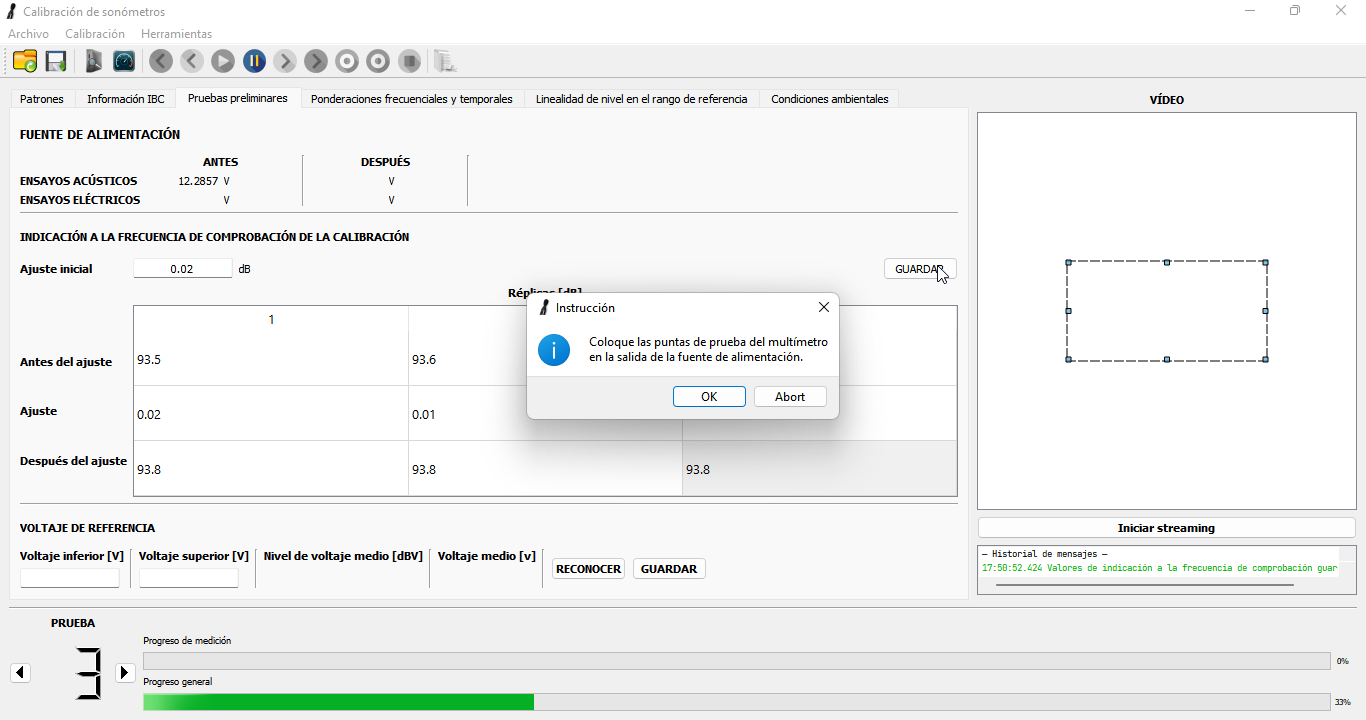
\includegraphics[width=0.9\textwidth]{4_implementación/Figs/slm_gui_results1}
    \caption*{\footnotesize Fuente: Elaboración propia.}
\end{figure}

\begin{figure}[!h]
    \centering
    \caption{Interfaz gráfica de usuario de la aplicación para sonómetros. Se muestra la pestaña de \emph{Pruebas preliminares} y la selección del área de interés sobre el vídeo.}
    \label{fig:slm_gui_results2}
    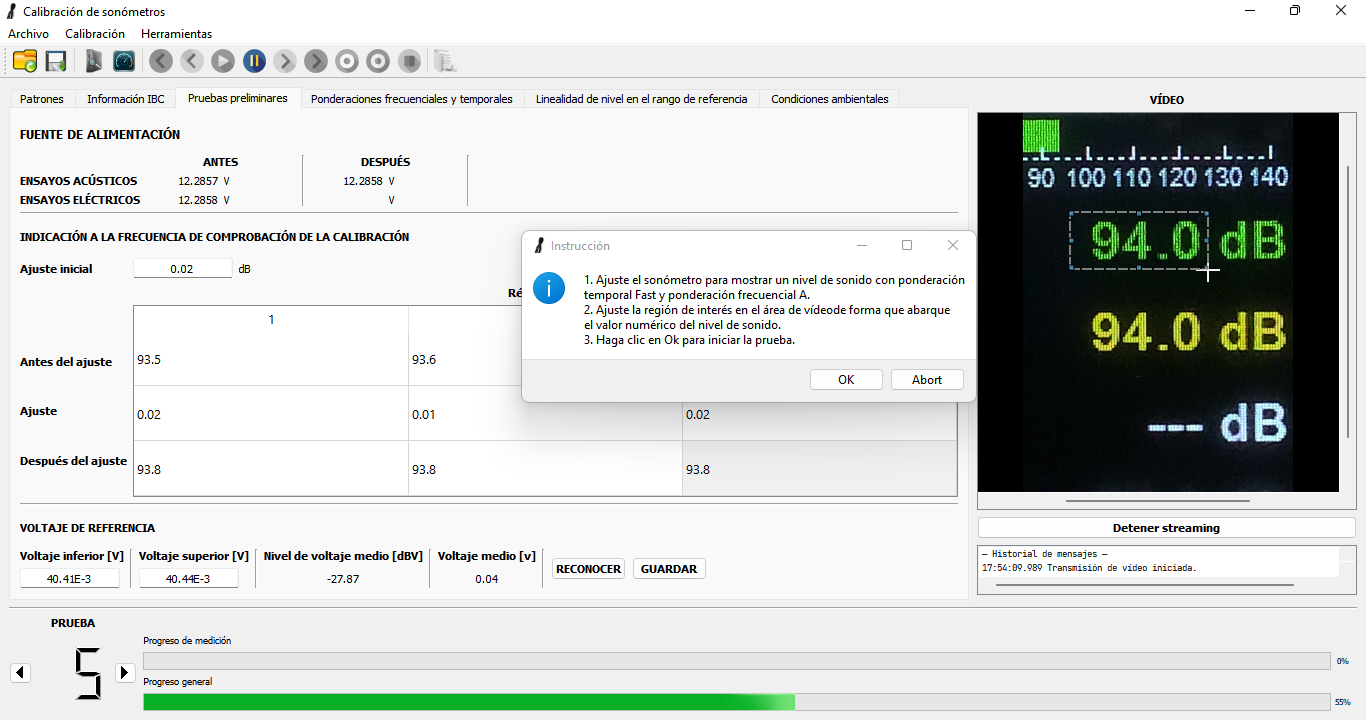
\includegraphics[width=0.9\textwidth]{4_implementación/Figs/slm_gui_results2}
    \caption*{\footnotesize Fuente: Elaboración propia.}
\end{figure}

\vfill
\clearpage

Al llegar al paso 5 (ponderación frecuencial $A$ con señales eléctricas), si no se ha activado la transmisión de vídeo, entonces esta iniciará y el usuario puede seleccionar el área de interés donde se encuentra el valor de medición que se desea reconocer (véase figura~\ref{fig:slm_gui_results2}).
Igualmente con las siguientes pruebas hasta el paso 10.
En la medida que avanzan las pruebas, los voltajes y frecuencias de las señales eléctricas se van ajustando automáticamente y se muestran en el historial los comandos SCPI enviados;
los resultados se presentan en tiempo real en sus campos correspondientes según la prueba en curso como se muestra en la siguiente figura.

\begin{figure}[!h]
    \centering
    \caption{Interfaz gráfica de usuario de la aplicación para sonómetros. Se muestra la pestaña de \emph{Ponderaciones frecuenciales y temporales} y la presentación de resultados.}
    \label{fig:slm_gui_results3}
    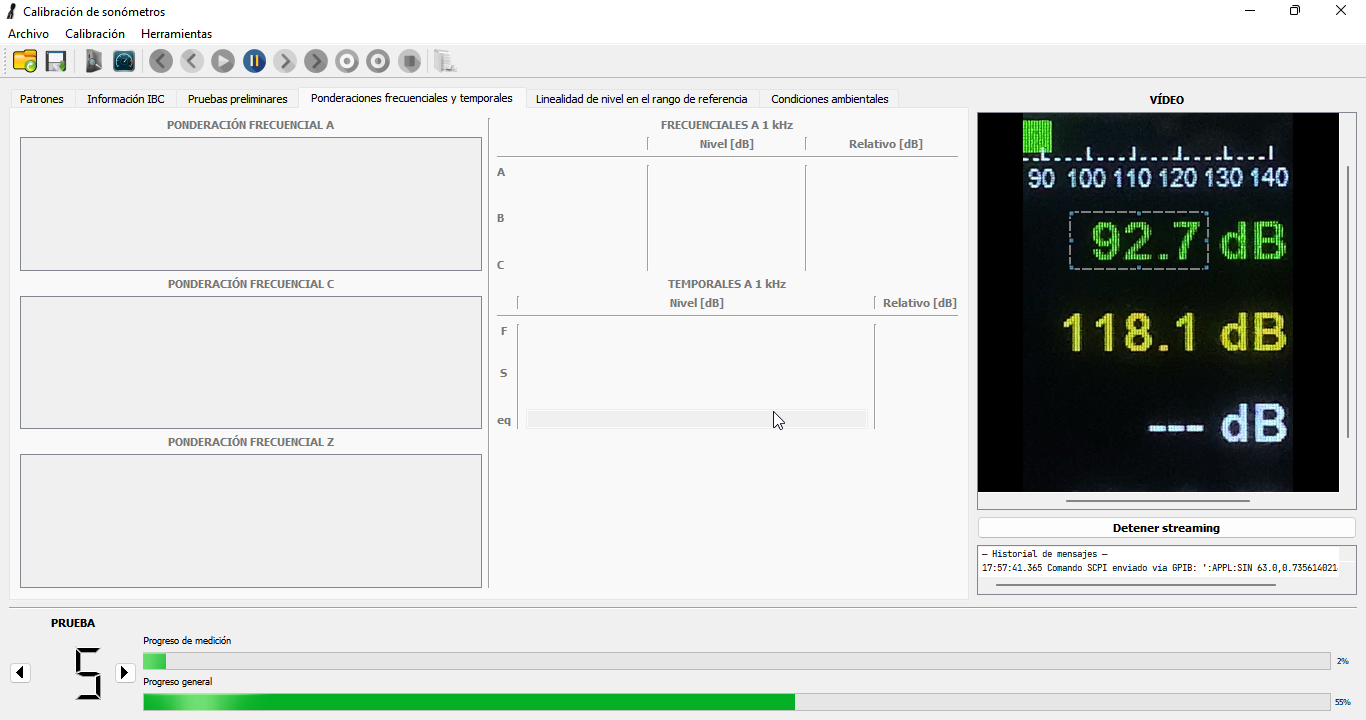
\includegraphics[width=\textwidth]{4_implementación/Figs/slm_gui_results3}
    \caption*{\footnotesize Fuente: Elaboración propia.}
\end{figure}

\vfill
\clearpage